\documentclass{article}

\usepackage[english]{babel} 
\usepackage[utf8]{inputenc}

\usepackage{amsfonts}
\usepackage{amsmath}
\usepackage{amssymb}
\usepackage{amsthm}
\usepackage{hyperref}
\usepackage[capitalize]{cleveref}
\usepackage{tikz}
\usetikzlibrary{knots, hobby}

\usepackage{graphicx}
\usepackage[a4paper, total={6in, 8in}]{geometry}

\newtheorem{thm}{Theorem}[section]
\newtheorem{lem}[thm]{Lemma}
\newtheorem{cor}[thm]{Corollary}
\newtheorem{prop}[thm]{Proposition}

\theoremstyle{definition}
\newtheorem{defi}[thm]{Definition}
\newtheorem{exa}[thm]{Example}
\newtheorem{exer}[thm]{Exercise}

\theoremstyle{remark}
\newtheorem{rem}[thm]{Remark}

\newcommand{\N}{\mathbb N}
\newcommand{\Z}{\mathbb Z}
\newcommand{\Q}{\mathbb Q}
\newcommand{\R}{\mathbb R}
\newcommand{\C}{\mathbb C}

\DeclareMathOperator{\crossing}{cr}

\title{Knots}
\author{Jack Haviland}
\date{14 July 2021}

\begin{document}

\maketitle

\section{What is a Knot?}

\begin{defi}
	A \emph{knot} is any closed loop in three-dimensional space. To think about this, you can imagine taking a piece of string and looping it around itself, then connecting the two loose ends to form a loop. Also, if we have a knot, we are allowed to move it around as long as the material doesn't pass through itself.
\end{defi}

The simplest knot is just a circle, and is called the \emph{unknot}. By moving the unknot around, we can make it look more complicated, but really it's still just the unknot.

It's very hard to talk about knots without being able to see them. To draw a knot, you can imagine placing the knot on a plane and tracing the loop. Of course, unless you have the unknot, there will have to be crossings in this tracing since the string can pass over and under itself. We indicate this by breaking the curve on the ``under'' strand, so it looks like the ``over'' strand is coming out of the page to pass over the crossing. Drawings of knots of this kind are called \emph{diagrams} or \emph{projections}.

\begin{figure}[h]
	\centering
	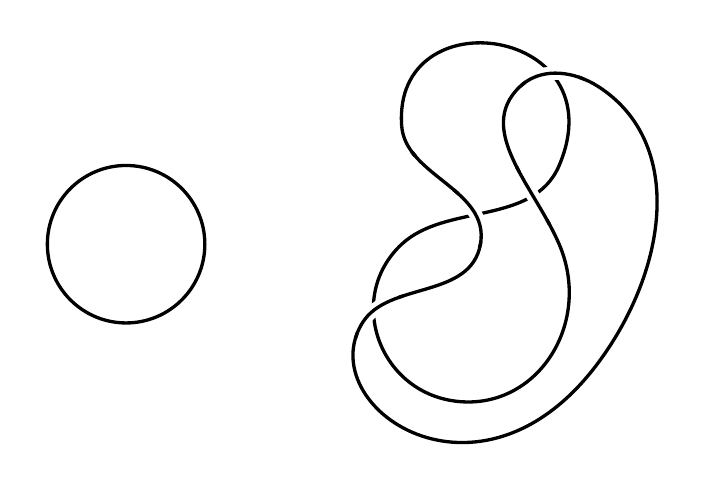
\begin{tikzpicture}[use Hobby shortcut]
		\useasboundingbox (-1.25, -2.75) rectangle (7,2.75);
		
		\draw[very thick] (0,0) circle (1);
		
		\begin{scope}[shift={(5,0)}]
			\begin{knot}[consider self intersections=true, ignore endpoint intersections=false, clip width=4]
				\coordinate (a) at (-1.5,1.5);
				\coordinate (b) at (-0.5,0);
				\coordinate (c) at (-2,-1);
				\coordinate (d) at (1,-1.5);
				\coordinate (e) at (1,2);
				\coordinate (f) at (0,2);
				\coordinate (g) at (0.5,0);
				\coordinate (h) at (-0.75,-2);
				\coordinate (i) at (-1.5,0);
				\coordinate (j) at (0.5,1);
				
				\strand[very thick] ([closed]a) .. (b) .. (c) .. (d) .. (e) .. (f) .. (g) .. (h) .. (i) .. (j) .. (a);
			\end{knot}
		\end{scope}
	\end{tikzpicture}
	\caption{Two drawings of the unknot}
	\label{fig:unknot}
\end{figure}

To see that the knot on the right is the unknot, you can imagine pulling the string tight and seeing that the crossings in the upper right ``cancel out'' and the crossing on the left ``cancel out,'' and all the crossings disappear. If you are not convinced by this argument, you can try making this knot out of real string and turning it into the drawing on the left.

\begin{exer}
	Draw a very complicated diagram of the unknot.
\end{exer}

\begin{exa}\label{exa:knots}
	Here are some more knots. Notice that you can't eliminate the crossings in any of the diagrams by pulling the string over itself, so these are genuinely different than the unknot. Of course, this is not a rigorous proof, but we will soon be able to prove that one of these knots is not the unknot.
	\begin{center}
		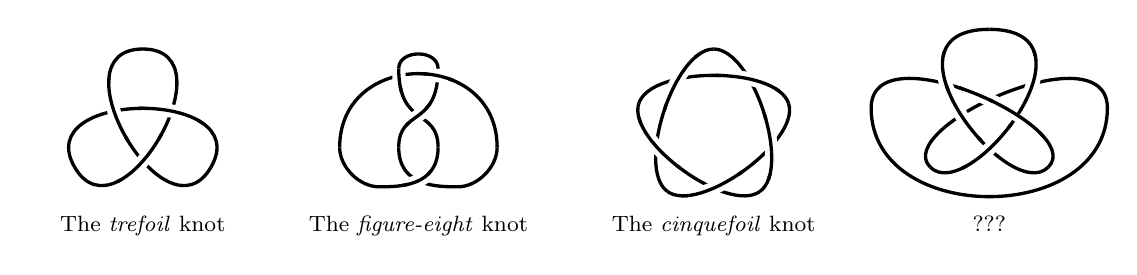
\begin{tikzpicture}
			
			\begin{scope}[shift={(3,0)}]
			\begin{knot}[clip width=4, flip crossing=1, flip crossing=3]
				\coordinate (t) at (90:1);
				\coordinate (l) at (210:1);
				\coordinate (r) at (330:1);
				
				\strand[very thick] (l) .. controls +(120:1.15) and +(60:1.15) .. (r);
				\strand[very thick] (r) .. controls +(240:1.15) and +(180:1.15) .. (t);
				\strand[very thick] (t) .. controls +(0:1.15) and +(300:1.15) .. (l);
			\end{knot}
			\node[below] at (0,-1) {\footnotesize The \emph{trefoil} knot};
			\end{scope}
			
			\begin{scope}[shift={(6.5,-0.25)}]
			\begin{knot}[clip width=4, flip crossing=2, flip crossing=3, clip radius=4pt, end tolerance=1pt]
				\coordinate (l) at (-1,0);
				\coordinate (r) at (1,0);
				\coordinate (tl) at (-0.25,1);
				\coordinate (tr) at (0.25,1);
				\coordinate (ml) at (-0.25,0);
				\coordinate (mr) at (0.25,0);
				\coordinate (bl) at (-0.5,-0.5);
				\coordinate (br) at (0.5,-0.5);
				
				\strand[very thick] (l) .. controls +(0,1.25) and +(0,1.25) .. (r);
				\strand[very thick] (r) .. controls +(0,-0.25) and +(0.25,0) .. (br);
				\strand[very thick] (br) .. controls +(-0.25,0) and +(0,-0.5) .. (ml);
				\strand[very thick] (ml) .. controls +(0,0.5) and +(0,-0.75) .. (tr);
				\strand[very thick] (tr) .. controls +(0,0.25) and +(0,0.25) .. (tl);
				\strand[very thick] (tl) .. controls +(0,-0.75) and +(0,0.5) .. (mr);
				\strand[very thick] (mr) .. controls +(0,-0.5) and +(0.25,0) .. (bl);
				\strand[very thick] (bl) .. controls +(-0.25,0) and +(0,-0.25) .. (l);
			\end{knot}
			\node[below] at (0,-0.75) {\footnotesize The \emph{figure-eight} knot};
			\end{scope}
			
			\begin{scope}[shift={(10.25,0)}]
				\begin{knot}[clip width=4, flip crossing=2, flip crossing=4]
					\coordinate (tr) at (18:1);
					\coordinate (t) at (90:1);
					\coordinate (tl) at (162:1);
					\coordinate (bl) at (-126:1);
					\coordinate (br) at (-54:1);
					
					\strand[very thick] (tr) .. controls +(108:0.5) and +(72:0.5) .. (tl);
					\strand[very thick] (tl) .. controls +(252:0.5) and +(-144:0.5) .. (br);
					\strand[very thick] (br) .. controls +(36:0.5) and +(0:0.5) .. (t);
					\strand[very thick] (t) .. controls +(180:0.5) and +(-216:0.5) .. (bl);
					\strand[very thick] (bl) .. controls +(-36:0.5) and +(-72:0.5) .. (tr);
				\end{knot}
				\node[below] at (0,-1) {\footnotesize The \emph{cinquefoil} knot};
			\end{scope}
			
			\begin{scope}[shift={(13.75,0.25)}]
				\begin{knot}[clip width=4, flip crossing=2, flip crossing=5, flip crossing=4, flip crossing=6]
					\coordinate (l) at (-1.5,0);
					\coordinate (r) at (1.5,0);
					\coordinate (ml) at (-0.75,-0.75);
					\coordinate (mr) at (0.75,-0.75);
					\coordinate (t) at (0,1);
					
					\strand[very thick] (l) .. controls +(0,-1.5) and +(0,-1.5) .. (r);
					\strand[very thick] (l) .. controls +(0, 1) and +(0.5,0.5) .. (mr);
					\strand[very thick] (r) .. controls +(0,1) and +(-0.5,0.5) .. (ml);
					\strand[very thick] (mr) .. controls +(-0.5,-0.5) and +(-1.5,0) .. (t);
					\strand[very thick] (ml) .. controls +(0.5,-0.5) and +(1.5,0) .. (t);
				\end{knot}
				\node[below] at (0,-1.25) {\footnotesize ???};
			\end{scope}
		\end{tikzpicture}
	\end{center}
\end{exa}

\section{Different Diagrams for the Same Knot}

We saw in the last section that different diagrams for the same knot can look very different. A natural question to ask, then, is how we can tell if two diagrams represent the same knot.

\begin{rem}
	Note that we are differentiating between a knot and a diagram for a knot. A knot is an object in three dimensions, while a diagram is a representation of a knot in two dimensions. In particular, there are many different diagrams for every knot.
\end{rem}

To answer this question, it would be helpful to understand how we can transform one diagram of a knot into another diagram of the same knot. These transformations correspond to moving the knot in three dimensions in a way that changes the projection. \emph{Reidemeister moves} are examples of this kind of transformation. There are three types, called type I, type II, and type III.

With type I, we can resolve a place where a strand loops back on itself. For the corresponding move in three dimensions, you can imagine flipping the loop over in a way that undoes the loop, removing the crossing. Adding such a loop is also considered a type I move, which does the opposite transformation.
\begin{center}
	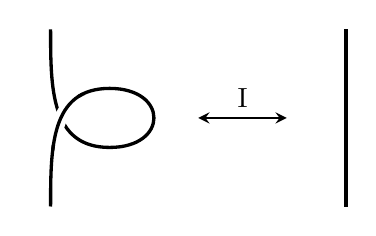
\begin{tikzpicture}[scale=0.75]
		\begin{knot}[clip width=4, consider self intersections=true]
			\strand[very thick] (0,0) .. controls +(0,1) and +(-1,0) .. (1,2) .. controls +(1,0) and +(1,0) .. (1,1) .. controls +(-1,0) and +(0,-1) .. (0,3);
			\draw[stealth-stealth, thick] (2.5,1.5) to node[midway, above] {I} (4,1.5);
			\strand[very thick] (5,0) -- (5,3);
		\end{knot}
	\end{tikzpicture}
\end{center}

In a type II move, we look at two strands where one has been placed on top  of the other. By pulling the strands apart, we can resolve both crossings simultaneously because the crossings ``cancel out,'' like we saw in \cref{fig:unknot}. For the corresponding move in three dimensions, you can imagine pulling the two strands apart so that the strand on top passes over the bottom strand. Given two adjacent strands that do not cross, adding two crossings in this way is also considered a type II move and does the opposite transformation.

\begin{center}
	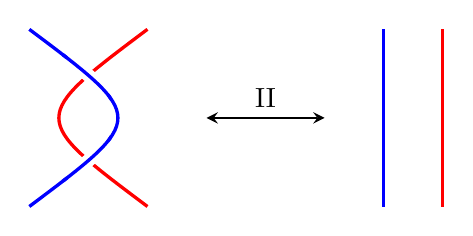
\begin{tikzpicture}[scale=0.75]
		\begin{knot}[clip width=4]
			\strand[very thick, blue] (0,0) .. controls +(2,1.5) and +(2,-1.5) .. (0,3);
			\strand[very thick, red] (2,0) .. controls +(-2,1.5) and +(-2,-1.5) .. (2,3);
			\draw[stealth-stealth, thick] (3,1.5) to node[midway, above] {II} (5,1.5);
			\strand[very thick, blue] (6,0) -- (6,3);
			\strand[very thick, red] (7,0) -- (7,3);
		\end{knot}
	\end{tikzpicture}
\end{center}

Finally, in a type III move, we start with three strands where each pair of strands crosses exactly once. One strand is ``over'' in both its crossings, one is ``under'' in both its crossings, and one has one of each type of crossing. For the type III move, you can either imagine passing the double-over strand on top of the crossing it is not involved in, or passing the double-under stand underneath the crossing it is not involved in. These respectively correspond to the blue and green strands below, and so you can see that the two ways to think about the move are equivalent. We can move the strand in either direction across the crossing to get two opposite kinds of type III moves.

\begin{center}
	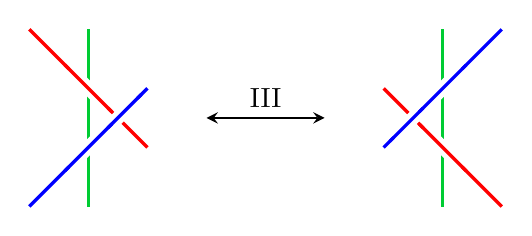
\begin{tikzpicture}[scale=0.75]
		\begin{knot}[clip width=4]
			\strand[very thick, blue] (0,0) -- (2,2);
			\strand[very thick, red] (0,3) -- (2,1);
			\strand[very thick, green!80!blue] (1,0) -- (1,3);
			\draw[stealth-stealth, thick] (3,1.5) to node[midway, above] {III} (5,1.5);
			\strand[very thick, blue] (6,1) -- (8,3);
			\strand[very thick, red] (6,2) -- (8,0);
			\strand[very thick, green!80!blue] (7,0) -- (7,3);
		\end{knot}
	\end{tikzpicture}
\end{center}

All of the Reidemeister moves are ``local,'' meaning it doesn't matter what the strands are doing in the rest of the knot, it just matters that in a small region, the strands match the pattern for the move.

\begin{exa}\label{exa:reidemeister}
	Let's use Reiemeister moves to turn something complicated into the unknot.
	\begin{center}
		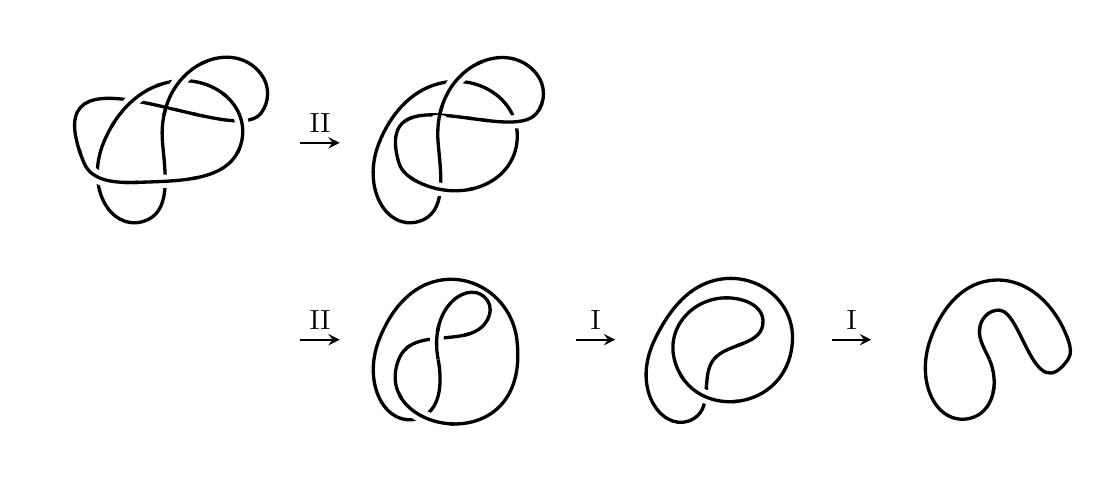
\begin{tikzpicture}[use Hobby shortcut, scale=0.5]
		\begin{scope}[shift={(0,0)}]
			\begin{knot}[clip width=4,
					consider self intersections=true,
					ignore endpoint intersections=false,
%					draft mode=crossings,
					flip crossing/.list={1,5,6}]
				\coordinate (a) at (-0.5,0);
				\coordinate (b) at (2,1.75);
				\coordinate (c) at (2,0.75);
				\coordinate (d) at (-2.5,-0.5);
				\coordinate (e) at (-1,-1);
				\coordinate (f) at (1.5,0);
				\coordinate (g) at (-0.5,1.5);
				\coordinate (h) at (-2,0);
				\coordinate (i) at (-1,-2);
				
%				\foreach \pt in {a,...,i} \node at (\pt){\pt};
				
				\strand[very thick] ([closed]a) .. (b) .. (c) .. (d) .. (e) .. (f) .. (g) .. (h) .. (i);
			\end{knot}
		\end{scope}
		
		\draw[thick, -stealth] (3,0) to node[above] {II} (4,0);
		
		\begin{scope}[shift={(7,0)}]
			\begin{knot}[clip width=4,
					consider self intersections=true,
					ignore endpoint intersections=false,
%					draft mode=crossings,
					flip crossing/.list={1}]
				\coordinate (a) at (-0.5,0);
				\coordinate (b) at (2,1.75);
				\coordinate (c) at (2,0.75);
				\coordinate (d) at (-1.5,-0.5);
				\coordinate (e) at (-1,-1);
				\coordinate (f) at (1.5,0);
				\coordinate (g) at (-0.5,1.5);
				\coordinate (h) at (-2,0);
				\coordinate (i) at (-1,-2);
				
%				\foreach \pt in {a,...,i} \node at (\pt){\pt};
				
				\strand[very thick] ([closed]a) .. (b) .. (c) .. (d) .. (e) .. (f) .. (g) .. (h) .. (i);
			\end{knot}
		\end{scope}
		
		\draw[thick, -stealth] (3,-5) to node[above] {II} (4,-5);
		
		\begin{scope}[shift={(7,-5)}]
			\begin{knot}[clip width=4,
					consider self intersections=true,
					ignore endpoint intersections=false,
%					draft mode=crossings,
					flip crossing/.list={1}]
				\coordinate (a) at (-0.5,-0.5);
				\coordinate (b) at (0.75,1);
				\coordinate (c) at (0.75,0.5);
				\coordinate (d) at (-1.5,-0.5);
				\coordinate (e) at (1.5,0);
				\coordinate (f) at (-0.5,1.5);
				\coordinate (g) at (-2,0);
				\coordinate (h) at (-1,-2);
				
%				\foreach \pt in {a,...,i} \node at (\pt){\pt};
				
				\strand[very thick] ([closed]a) .. (b) .. (c) .. (d) .. (e) .. (f) .. (g) .. (h);
			\end{knot}
		\end{scope}
		
		\draw[thick, -stealth] (10,-5) to node[above] {I} (11,-5);
		
		\begin{scope}[shift={(14,-5)}]
			\begin{knot}[clip width=4,
					consider self intersections=true,
					ignore endpoint intersections=false,
%					draft mode=crossings,
					flip crossing/.list={1}]
				\coordinate (a) at (-0.5,-0.5);
				\coordinate (b) at (0.75,0.5);
				\coordinate (c) at (0.25,1);
				\coordinate (d) at (-1.5,-0.5);
				\coordinate (e) at (1.5,0);
				\coordinate (f) at (-0.5,1.5);
				\coordinate (g) at (-2,0);
				\coordinate (h) at (-1,-2);
				
%				\foreach \pt in {a,...,i} \node at (\pt){\pt};
				
				\strand[very thick] ([closed]a) .. (b) .. (c) .. (d) .. (e) .. (f) .. (g) .. (h);
			\end{knot}
		\end{scope}
		
		\draw[thick, -stealth] (16.5,-5) to node[above] {I} (17.5,-5);
		
		\begin{scope}[shift={(21,-5)}]
			\begin{knot}[clip width=4,
					consider self intersections=true,
					ignore endpoint intersections=false,
%					draft mode=crossings,
					flip crossing/.list={1}]
				\coordinate (a) at (-0.5,-0.5);
				\coordinate (b) at (-0.75,0.25);
				\coordinate (c) at (-0.25,0.75);
				\coordinate (d) at (1.5,-0.5);
				\coordinate (e) at (1.5,0);
				\coordinate (f) at (-0.5,1.5);
				\coordinate (g) at (-2,0);
				\coordinate (h) at (-1,-2);
				
%				\foreach \pt in {a,...,i} \node at (\pt){\pt};
				
				\strand[very thick] ([closed]a) .. (b) .. (c) .. (d) .. (e) .. (f) .. (g) .. (h);
			\end{knot}
		\end{scope}
		\end{tikzpicture}
	\end{center}
	This shows that we just have a complicated diagram for the unknot again!
\end{exa}

\begin{exer}
	Can you find a shorter sequence of Reidemeister moves that transforms the diagram in \cref{exa:reidemeister} to the trivial diagram of the unknot?
\end{exer}

\begin{exer}
	Find a sequence of Reidemeister moves that transforms the ``???'' knot in \cref{exa:knots} to the trefoil knot.
\end{exer}

The Reidemeister moves are special and important because of the following miraculous theorem proved by Kurt Reidemeister in 1926.

\begin{thm}[Reidemeister, 1926]
	Any two diagrams representing the same knot are related by a sequence of Reidemeister moves.\qed
\end{thm}

Proving this theorem is rather involved and we will not do it here. For those interested, Kauffman \cite{K} gives a summary of the techniques Reidemeister used to prove his theorem. Note, however, that statements of Reidemeister's theorem in modern treatments of knot theory require stronger methods from algebraic topology.

Reidemeister's theorem gives us an ``if and only if'' criterion for knowing when two diagrams represent the same knot. However, it's not really feasible to prove two diagrams represent different knots by proving that there is no sequence of Reidemeister moves to get from one to the other because there are infinitely many possible sequences of Reidemeister moves. So, in order to prove that knots are different, we will need a different idea.

\section{Knot Invariants}

The way we will tell knots apart is with \emph{invariants}. For our purposes, an invariant is a property that is the same for all diagrams of a knot. The first we will discuss is crossing number.

\begin{defi}
	The \emph{crossing number} of a knot diagram is the number of crossings in the diagram. If $D$ is a knot diagram, we denote the crossing number of $D$ by $\tilde \crossing(D)$.
\end{defi}

Crossing number is a natural measure of the complexity of a knot diagram, since diagrams with more crossings are visually more complex than those with fewer crossings. However, crossing number is not an invariant. We've already seen diagrams for the unknot that have crossing numbers $0$, $4$, and $6$. In order to make crossing number an invariant, we need to take the minimum crossing number over all possible diagrams of a knot. Formally, if $K$ is a knot, then we define the crossing number of $K$ to be
\[
\crossing(K) = \min \{\tilde \crossing(D) \mid D \text{ is a diagram of } K\}.
\]
Notice the difference between the crossing number of a diagram compared to the crossing number of a knot. Both measure complexity, but the crossing number of a diagram measures complexity of a single diagram while crossing number of a knot measures complexity of the underlying knot.

\begin{exa}
	The crossing numbers for the diagrams in \cref{exa:knots} are $0$ for the unknot, $3$ for the trefoil knot, $4$ for the figure-eight knot, $5$ for the cinquefoil knot, and $6$ for the ??? knot. In fact, for the unknot, trefoil knot, figure-eight knot, and cinquefoil knot, these are the crossing numbers of the knots themselves as well.
\end{exa}

\begin{exa}
	There are no knots with crossing number $1$ or $2$. Equivalently, every diagram with one or two crossings can be simplified to the unknot. To prove this, we can just look at all the diagrams with one or two crossings. For one crossing, we can start with the strands of the crossings and look at ways to connect them in a way that creates a one-crossing knot diagram. 
	
	\begin{figure}[h]
		\centering
		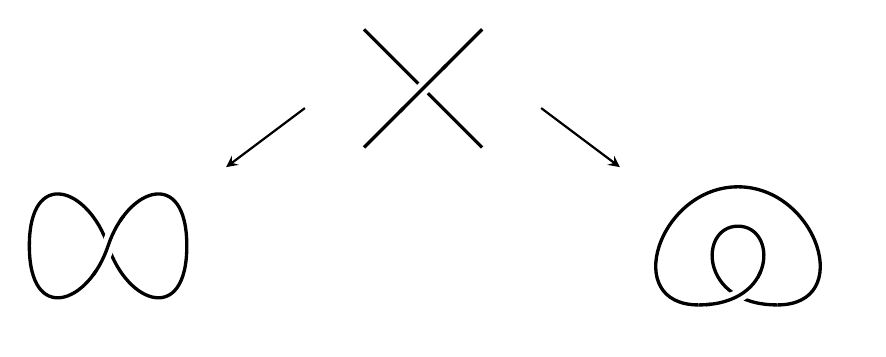
\begin{tikzpicture}
			\begin{knot}[clip width=4]
				\strand[very thick] (-0.75,-0.75) -- (0.75,0.75);
				\strand[very thick] (-0.75,0.75) -- (0.75,-0.75);
			\end{knot}
			
			\begin{scope}[shift={(-4,-2)}]
			\begin{knot}[clip width=4, flip crossing=1]
				\strand[very thick] (-1,0) .. controls +(0,1) and +(-0.25,0.75) .. (0,0) .. controls +(0.25,-0.75) and +(0,-1) .. (1,0);
				\strand[very thick] (-1,0) .. controls +(0,-1) and +(-0.25,-0.75) .. (0,0) .. controls +(0.25,0.75) and +(0,1) .. (1,0);
			\end{knot}
			\end{scope}
			
			\begin{scope}[shift={(4,1.25)}]
			\begin{knot}[clip width=4, end tolerance=2pt]
				\strand[very thick] (-0.5,-4) .. controls +(1,0) and +(0.5,0) .. (0,-3);
				\strand[very thick] (0,-3) .. controls +(-0.5,0) and +(-1,0) .. (0.5,-4);
				\strand[very thick] (0.5,-4) .. controls +(1,0) and +(1,0) .. (0,-2.5) .. controls +(-1,0) and +(-1,0) .. (-0.5,-4);
			\end{knot}
			\end{scope}
			
			\draw[thick, -stealth] (-1.5,-0.25) -- (-2.5,-1);
			\draw[thick, -stealth] (1.5,-0.25) -- (2.5,-1);
		\end{tikzpicture}
		\caption{The only one-crossing knot diagrams}
		\label{fig:one crossing}
	\end{figure}
	
	Any other way of connecting the strands either results in a rotation of one of the diagrams in \cref{fig:one crossing} or creates more crossings, so up to rotation these are the only two diagrams with one crossing. In each case, we can apply a type I Reidemeister move to obtain a diagram of the unknot, proving that there are not knots of crossing number $1$.
	
	Similarly, but with more involved casework, one can show that the only diagrams with two crossings are rotations and reflections of those in \cref{fig:two crossing}. In all cases, we can apply a type I move to obtain a diagram with one crossing, so all the diagrams must represent the unknot.
	
	\begin{figure}[h]
		\centering
		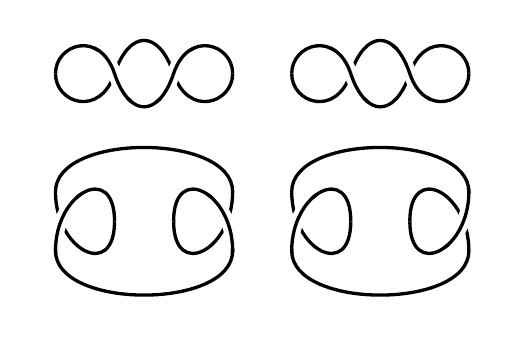
\begin{tikzpicture}[scale=0.75]
			\begin{scope}[shift={(0,0)}]
			\begin{knot}[clip width=4]
				\strand[very thick] (-2,0) .. controls +(0,0.5) and +(-0.25,0.75) .. (-1,0) .. controls +(0.25,-0.75) and +(-0.25,-0.75) .. (0,0) .. controls +(0.25,0.75) and +(0,0.5) .. (1,0);
				\strand[very thick] (-2,0) .. controls +(0,-0.5) and +(-0.25,-0.75) .. (-1,0) .. controls +(0.25,0.75) and +(-0.25,0.75) .. (0,0) .. controls +(0.25,-0.75) and +(0,-0.5) .. (1,0);
			\end{knot}
			\end{scope}
			
			
			\begin{scope}[shift={(4,0)}]
			\begin{knot}[clip width=4, flip crossing=2]
				\strand[very thick] (-2,0) .. controls +(0,0.5) and +(-0.25,0.75) .. (-1,0) .. controls +(0.25,-0.75) and +(-0.25,-0.75) .. (0,0) .. controls +(0.25,0.75) and +(0,0.5) .. (1,0);
				\strand[very thick] (-2,0) .. controls +(0,-0.5) and +(-0.25,-0.75) .. (-1,0) .. controls +(0.25,0.75) and +(-0.25,0.75) .. (0,0) .. controls +(0.25,-0.75) and +(0,-0.5) .. (1,0);
			\end{knot}
			\end{scope}
			
			\begin{scope}[shift={(0,-2.5)}]
			\begin{knot}[clip width=4]
				\strand[very thick] (-1,0) .. controls +(0,1) and +(0,1) .. (-2,-0.5) .. controls +(0,-1) and +(0,-1) .. (1,-0.5) .. controls +(0,1) and +(0,1) .. (0,0);
				\strand[very thick] (-1,0) .. controls +(0,-1) and +(0,-1) .. (-2,0.5) .. controls +(0,1) and +(0,1) .. (1,0.5) .. controls +(0,-1) and +(0,-1) .. (0,0);
			\end{knot}
			\end{scope}
			
			\begin{scope}[shift={(4,-2.5)}]
			\begin{knot}[clip width=4, flip crossing=2]
				\strand[very thick] (-1,0) .. controls +(0,1) and +(0,1) .. (-2,-0.5) .. controls +(0,-1) and +(0,-1) .. (1,-0.5) .. controls +(0,1) and +(0,1) .. (0,0);
				\strand[very thick] (-1,0) .. controls +(0,-1) and +(0,-1) .. (-2,0.5) .. controls +(0,1) and +(0,1) .. (1,0.5) .. controls +(0,-1) and +(0,-1) .. (0,0);
			\end{knot}
			\end{scope}
		\end{tikzpicture}
		\caption{The only two-crossing knot diagrams}
		\label{fig:two crossing}
	\end{figure}
\end{exa}

Since crossing number is a good measure of complexity, it is usually used in tables of knots (complete lists of distinct knots) to categorize the knots listed and give some kind of order to the presentation.

Next, we'll look at invariant that does a better job distinguishing between different knots.

\begin{defi}
	A knot diagram is \emph{tricolorable} if, using three colors, we can assign a color to each strand in such a way that at least two colors are used and at each crossing, either all three strands are the same color or all three strands are different colors.
\end{defi}

\begin{figure}[h]
	\centering
	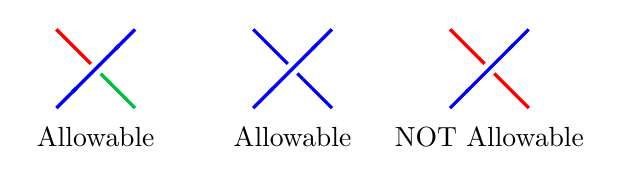
\begin{tikzpicture}[scale=0.5]
		\begin{knot}[clip width=4, end tolerance=0pt]
			\strand[very thick, blue] (-1,-1) -- (1,1);
			\strand[very thick, red] (-1,1) -- (0,0);
			\strand[very thick, green!75!blue] (0,0) -- (1,-1);
			\node[below] at (0,-1.25) {Allowable};
		\end{knot}
		
		\begin{scope}[shift={(5,0)}]
		\begin{knot}[clip width=4]
			\strand[very thick, blue] (-1,-1) -- (1,1);
			\strand[very thick, blue] (-1,1) -- (1,-1);
			\node[below] at (0,-1.25) {Allowable};
		\end{knot}
		\end{scope}
		
		\begin{scope}[shift={(10,0)}]
		\begin{knot}[clip width=4]
			\strand[very thick, blue] (-1,-1) -- (1,1);
			\strand[very thick, red] (-1,1) -- (1,-1);
			\node[below] at (0,-1.25) {NOT Allowable};
		\end{knot}
		\end{scope}
	\end{tikzpicture}
	\caption{Allowability of crossings for tricoloring}
	\label{fig:tricolor}
\end{figure}

In \cref{fig:tricolor}, the first and second crossings are both allowable by definition. However, third crossing is not allowable because it has two red strands, but not all the strands are red. Note that not every crossing can be like the second crossing because at least two colors must be used.

\begin{exa}\label{exa:tricolor unknot}
	Let's look at several diagrams of the unknot to see if they can be tricolored.
	\begin{center}
		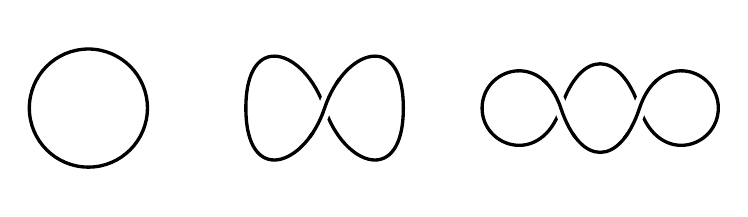
\begin{tikzpicture}
			\draw[very thick] (-5,0) circle (0.75);
			
			\begin{scope}[shift={(-2,0)}]
			\begin{knot}[clip width=4, flip crossing=1]
				\strand[very thick] (-1,0) .. controls +(0,1) and +(-0.25,0.75) .. (0,0) .. controls +(0.25,-0.75) and +(0,-1) .. (1,0);
				\strand[very thick] (-1,0) .. controls +(0,-1) and +(-0.25,-0.75) .. (0,0) .. controls +(0.25,0.75) and +(0,1) .. (1,0);
			\end{knot}
			\end{scope}
			
			\begin{scope}[shift={(2,0)}]
			\begin{knot}[clip width=4]
				\strand[very thick] (-2,0) .. controls +(0,0.5) and +(-0.25,0.75) .. (-1,0) .. controls +(0.25,-0.75) and +(-0.25,-0.75) .. (0,0) .. controls +(0.25,0.75) and +(0,0.5) .. (1,0);
				\strand[very thick] (-2,0) .. controls +(0,-0.5) and +(-0.25,-0.75) .. (-1,0) .. controls +(0.25,0.75) and +(-0.25,0.75) .. (0,0) .. controls +(0.25,-0.75) and +(0,-0.5) .. (1,0);
			\end{knot}
			\end{scope}
		\end{tikzpicture}
	\end{center}
	The first cannot be tricolored because there is no way to use more than one color (there is only one strand). The same holds for the second diagram, which also has only one strand. For the third diagram, if we start by coloring the ``long'' strand any color, say blue, then at each crossing there will be two blue strands, so the third strand also has to be blue (otherwise, the crossing would not be allowable). Therefore the other strand must be colored the same, but this means we cannot use two different colors. Thus, none of the diagrams can be tricolored.
\end{exa}

If we want to use tricolorability as an invariant, we need to know that either every diagram of a knot is tricolorable or no diagram of the knot is tricolorable. To prove this, we will prove that Reidemeister moves don't change tricolorability. Then, if any diagram of a knot is tricolorable, we could apply Reidemeister moves to get to any other diagram and see that every diagram of the knot is tricolorable. On the other hand, if any diagram is not tricolorable, no diagram can be tricolorable because otherwise we could apply Reidemeister moves to obtain a tricoloring of the non-tricolorable diagram. Crucially, this gives us a way to tell that two diagrams represent different knots. Namely, if one diagram is tricolorable and the other is not, then they cannot represent the same knot.

\begin{thm}
	Tricolorability is preserved by Reidemeister moves.
\end{thm}

\begin{proof}
	We will prove this by casework for each of the three types of moves. For type I, if either side appears in a tricolored knot diagram, then everything must be the same color. On the right, this is clear because there is only one strand. On the left, if the over strand has any color, say blue, then the crossing will have two blue strands and so the remaining strand must also be blue. So indeed, in both cases everything must be the same color. Moreover, since everything is the same color, another color must appear elsewhere in the tricoloring. Hence we can just perform the type I move in either direction and keep all the colors the same, and the resulting diagram will be tricolored.
	
	\begin{center}
		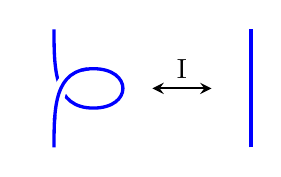
\begin{tikzpicture}[scale=0.5]
			\begin{knot}[clip width=4, consider self intersections=true]
				\strand[very thick, blue] (0,0) .. controls +(0,1) and +(-1,0) .. (1,2) .. controls +(1,0) and +(1,0) .. (1,1) .. controls +(-1,0) and +(0,-1) .. (0,3);
				\draw[stealth-stealth, thick] (2.5,1.5) to node[midway, above] {I} (4,1.5);
				\strand[very thick, blue] (5,0) -- (5,3);
			\end{knot}
		\end{tikzpicture}
	\end{center}
	
	For type II, there are two possible colorings up to switching colors:
	
	\begin{center}
		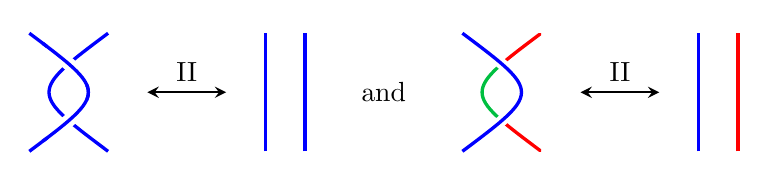
\begin{tikzpicture}[scale=0.5]
			\begin{knot}[clip width=4]
				\strand[very thick, blue] (0,0) .. controls +(2,1.5) and +(2,-1.5) .. (0,3);
				\strand[very thick, blue] (2,0) .. controls +(-2,1.5) and +(-2,-1.5) .. (2,3);
				\draw[stealth-stealth, thick] (3,1.5) to node[midway, above] {II} (5,1.5);
				\strand[very thick, blue] (6,0) -- (6,3);
				\strand[very thick, blue] (7,0) -- (7,3);
			\end{knot}
			
			\node at (9,1.5) {and};
			
			\begin{scope}[shift={(11,0)}]
				\begin{scope}
					\clip (1,0) rectangle (2,3);
					\draw[very thick, red] (2,0) .. controls +(-2,1.5) and +(-2,-1.5) .. (2,3);
				\end{scope}
				\begin{scope}
					\clip (0,0) rectangle (1,3);
					\draw[very thick, green!75!blue] (2,0) .. controls +(-2,1.5) and +(-2,-1.5) .. (2,3);
				\end{scope}
				\draw[line width=4, white] (0,0) .. controls +(2,1.5) and +(2,-1.5) .. (0,3);
				\draw[very thick, blue] (0,0) .. controls +(2,1.5) and +(2,-1.5) .. (0,3);
				
				\draw[stealth-stealth, thick] (3,1.5) to node[midway, above] {II} (5,1.5);
				\draw[very thick, blue] (6,0) -- (6,3);
				\draw[very thick, red] (7,0) -- (7,3);
			\end{scope}
		\end{tikzpicture}
	\end{center}
	
	Again, on the right this is clear because there are two strands to color. On the left, imagine first coloring the over strand blue, then choosing a color for the top right under strand. The color is either blue or something different; the colors of the other two strands are forced by creating a valid tricoloring in both cases and we obtain the two colorings shown. In either coloring case, we can start from either side, apply a type II move, and obtain a valid tricoloring of the new diagram. In the case when everything is the same color, another color must have appeared somewhere else in the original diagram, and this is unaffected by the move and new coloring. In the other case, both sides have at least two colors shown, so there is no need to worry about using at least two colors.
	
	Finally, for the type III move, there are five cases, which can be generated by coloring the double-over strand, then choosing to color the top part of the over-under strand either the same color, then choosing between either same/different (if the first two colors were the same) or between any of the three colors (if the first two colors were different). The rest of the colors are always forced by having a valid tricoloring at each crossing.

\newcommand{\reidIIIleft}[6]{
	% double-under
	% upper
	\begin{scope}
		\clip (0,3) -- (2,1) -- (2,3) -- cycle;
		\draw[very thick, #4] (1,0) -- (1,3);
	\end{scope}
	% middle
	\begin{scope}
		\clip (0,3) -- (1.5,1.5) -- (0,0) -- cycle;
		\draw[very thick, #5] (1,0) -- (1,3);
	\end{scope}
	% lower
	\begin{scope}
		\clip (0,0) -- (2,2) -- (2,0) -- cycle;
		\draw[very thick, #6] (1,0) -- (1,3);
	\end{scope}
	
	% over-under
	\draw[line width=4, white] (0,3) -- (2,1);
	% upper
	\begin{scope}
		\clip (-0.1,0) -- (2.1,2) -- (2.1,3.1) -- (-0.1,3.1) -- cycle;
		\draw[very thick, #2] (0,3) -- (2,1);
	\end{scope}
	% lower
	\begin{scope}
		\clip (0,0) -- (2.1,2) -- (2.1,0) -- cycle;
		\draw[very thick, #3] (0,3) -- (2,1);
	\end{scope}
	
	% double-over
	\draw[line width=4, white] (0,0) -- (2,2);
	\draw[very thick, #1] (0,0) -- (2,2);
}
\newcommand{\reidIIIright}[6]{
	\begin{scope}[shift={(5,0)}]
	% double-under
	% upper
	\begin{scope}
		\clip (0,1) -- (2.1,3.1) -- (0,3.1) -- cycle;
		\draw[very thick, #4] (1,0) -- (1,3);
	\end{scope}
	% middle
	\begin{scope}
		\clip (0.5,1.5) -- (2,3) -- (2,0) -- cycle;
		\draw[very thick, #5] (1,0) -- (1,3);
	\end{scope}
	% lower
	\begin{scope}
		\clip (0,2) -- (2,0) -- (0,0) -- cycle;
		\draw[very thick, #6] (1,0) -- (1,3);
	\end{scope}
	
	% over-under
	\draw[line width=4, white] (0,2) -- (2,0);
	% upper
	\begin{scope}
		\clip (-0.1,1) -- (2,3) -- (-0.1,3) -- cycle;
		\draw[very thick, #2] (0,2) -- (2,0);
	\end{scope}
	% lower
	\begin{scope}
		\clip (0,1) -- (2.1,3) -- (2.1,-0.1) -- (0,-0.1) -- cycle;
		\draw[very thick, #3] (0,2) -- (2,0);
	\end{scope}
	
	% double-over
	\draw[line width=4, white] (0,1) -- (2,3);
	\draw[very thick, #1] (0,1) -- (2,3);
	\end{scope}
}

	\begin{center}
		\begin{tikzpicture}[scale=0.5]
			\begin{scope}[shift={(0,-2)}]
				\reidIIIleft{blue}{blue}{blue}{blue}{blue}{blue}
				\draw[stealth-stealth, thick] (2.5,1.5) to node[midway, above] {III} (4.5,1.5);
				\reidIIIright{blue}{blue}{blue}{blue}{blue}{blue}
			\end{scope}
			
			\begin{scope}[shift={(0,-6)}]
				\reidIIIleft{blue}{blue}{blue}{red}{green!75!blue}{red}
				\draw[stealth-stealth, thick] (2.5,1.5) to node[midway, above] {III} (4.5,1.5);
				\reidIIIright{blue}{blue}{blue}{red}{green!75!blue}{red}
			\end{scope}

			
			\begin{scope}[shift={(12,0)}]
				\reidIIIleft{blue}{red}{green!75!blue}{blue}{green!75!blue}{red}\draw[stealth-stealth, thick] (2.5,1.5) to node[midway, above] {III} (4.5,1.5);
				\reidIIIright{blue}{red}{green!75!blue}{blue}{blue}{red}
			\end{scope}
			
			\begin{scope}[shift={(12,-4)}]
				\reidIIIleft{blue}{red}{green!75!blue}{red}{red}{green!75!blue}\draw[stealth-stealth, thick] (2.5,1.5) to node[midway, above] {III} (4.5,1.5);
				\reidIIIright{blue}{red}{green!75!blue}{red}{green!75!blue}{green!75!blue}
			\end{scope}
			
			\begin{scope}[shift={(12,-8)}]
				\reidIIIleft{blue}{red}{green!75!blue}{green!75!blue}{blue}{blue}\draw[stealth-stealth, thick] (2.5,1.5) to node[midway, above] {III} (4.5,1.5);
				\reidIIIright{blue}{red}{green!75!blue}{green!75!blue}{red}{blue}
			\end{scope}
		\end{tikzpicture}
	\end{center}
	
	As we saw with the type I and II moves, from any starting position we can apply a type III move and obtain a valid tricoloring of the resulting diagram. In every case except the first, we already have two distinct colors visible; in the first case, another color must appear somewhere else in the diagram for both the left and right starting positions.
	
	Note that in all three cases, whenever we applied a move and constructed a tricoloring of the resulting diagram, the changes were only local and did not affect the rest of the diagram because the strands leading out of the important crossings were left unchanged. Thus, we can apply any Reidemeister move to a tricolored knot diagram and obtain a tricoloring of the resulting diagram.
\end{proof}

This proves that it makes sense to talk about the tricolorability of a knot, rather than just a diagram. We will conclude by proving that the trefoil knot and the unknot are different.

\begin{cor}
	The unknot is not tricolorable.
\end{cor}

\begin{proof}
	We saw in \cref{exa:tricolor unknot} that there are several diagrams of the unknot which cannot be tricolored, hence no diagram can be tricolored.
\end{proof}

Thus, it suffices to show that the trefoil knot is tricolorable, and the best way to do this is to give an explicit tricoloring of a diagram. In \cref{fig:tricolor trefoil}, at each crossing there are three different colors, hence we have a valid tricoloring. This proves that the trefoil knot is not the unknot!

\begin{figure}[h]
	\centering
	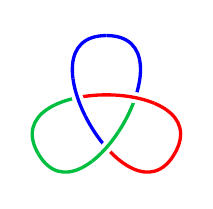
\begin{tikzpicture}
		\useasboundingbox (-1,-0.85) rectangle (1,1.1);
		\begin{knot}[clip width=4]
			\coordinate (t) at (90:1);
			\coordinate (l) at (210:1);
			\coordinate (r) at (330:1);
			
			\strand[very thick, draw=none] (l) .. controls +(120:1.15) and +(60:1.15) .. (r);
			\strand[very thick, draw=none] (r) .. controls +(240:1.15) and +(180:1.15) .. (t);
			\strand[very thick, draw=none] (t) .. controls +(0:1.15) and +(300:1.15) .. (l);
		\end{knot}
		% blue, left
		\begin{scope}
			\clip (t) .. controls +(0:1.15) and +(300:1.15) .. (l) -- +(0,1.75) -- +(1,1.75) -- cycle;
			\draw[very thick, blue] (r) .. controls +(240:1.15) and +(180:1.15) .. (t);
		\end{scope}
		
		% blue, right
		\begin{scope}
			\clip (l) .. controls +(120:1.15) and +(60:1.15) .. (r) -- +(0,1.75) -- +(-2,1.75) -- cycle;
			\draw[very thick, blue] (t) .. controls +(0:1.15) and +(300:1.15) .. (l);
		\end{scope}
		
		% red, upper
		\begin{scope}
			\clip (r) .. controls +(240:1.15) and +(180:1.15) .. (t) -- (1,1) -- (1,-0.6) -- cycle;
			\draw[very thick, red] (l) .. controls +(120:1.15) and +(60:1.15) .. (r);
		\end{scope}
		
		% red, lower
		\begin{scope}
			\clip (t) .. controls +(0:1.15) and +(300:1.15) .. (l) -- +(0,-0.5) -- +(2,-0.5) -- +(2,1.5) -- cycle;
			\draw[very thick, red] (r) .. controls +(240:1.15) and +(180:1.15) .. (t);
		\end{scope}
		
		% green, upper
		\begin{scope}
			\clip (r) .. controls +(240:1.15) and +(180:1.15) .. (t) -- (-1.2,1) -- (-1.2,-1) -- (0,-1) -- cycle;
			\draw[very thick, green!75!blue] (l) .. controls +(120:1.15) and +(60:1.15) .. (r);
		\end{scope}
		
		% green, lower
		\begin{scope}
			\clip (l) .. controls +(120:1.15) and +(60:1.15) .. (r) -- +(0,-0.5) -- + (-1.8,-0.5) -- +(-1.8,0.1) -- cycle;
			\draw[very thick, green!75!blue] (t) .. controls +(0:1.15) and +(300:1.15) .. (l);
		\end{scope}
		
		% crossings
		% blue over
		\begin{scope}
			\clip (knot 1.center) circle (0.25);
			\draw[line width=4, white] (r) .. controls +(240:1.15) and +(180:1.15) .. (t);
			\draw[very thick, blue] (r) .. controls +(240:1.15) and +(180:1.15) .. (t);
		\end{scope}
		
		% red over
		\begin{scope}
			\clip (knot 2.center) circle (0.25);
			\draw[line width=4, white] (l) .. controls +(120:1.15) and +(60:1.15) .. (r);
			\draw[very thick, red] (l) .. controls +(120:1.15) and +(60:1.15) .. (r);
		\end{scope}
		
		% green over
		\begin{scope}
			\clip (knot 3.center) circle (0.25);
			\draw[line width=4, white] (t) .. controls +(0:1.15) and +(300:1.15) .. (l);
			\draw[very thick, green!75!blue] (t) .. controls +(0:1.15) and +(300:1.15) .. (l);
		\end{scope}
	\end{tikzpicture}
	\caption{Tricoloring a trefoil knot}
	\label{fig:tricolor trefoil}
\end{figure}

\begin{exer}
	When defining tricolorability, we could have used the three digits $0, 1, 2$ instead of three colors. Rewrite the tricolorability criterion as an equation in $\Z_3$ that must be satisfied by the labels of the over and under strands at each crossing. Can you generalize?
\end{exer}

\begin{exer}
	Prove that the figure-eight knot is not the unknot.
\end{exer}

\begin{thebibliography}{99}
	\bibitem[K]{K} Kauffman, Louis H. Knot diagrammatics. \emph{Handbook of knot theory}, 233–318, \emph{Elsevier B. V.}, \emph{Amsterdam}, 2005 \href{https://arxiv.org/abs/math/0410329}{https://arxiv.org/abs/math/0410329}
\end{thebibliography}


\end{document}
